{\fontsize{12pt}{22pt} \textbf{AdaBoost}\par}

\vspace{5mm}

Boosting is an algorithmic paradigm addressing two major issues in machine learning:

- It optimizes the \hyperref[sec:bias-complexity-trade-off]{bias-complexity trade-off}. The learning starts with a basic class (large approximation error) and as it progresses the hypothesis class becomes more complex.

- It allows to find predictors that are usually computationally infeasible to find.

\vspace{5mm}

Main idea: weak learners are "boosted" to become stronger altogether.

\begin{center}
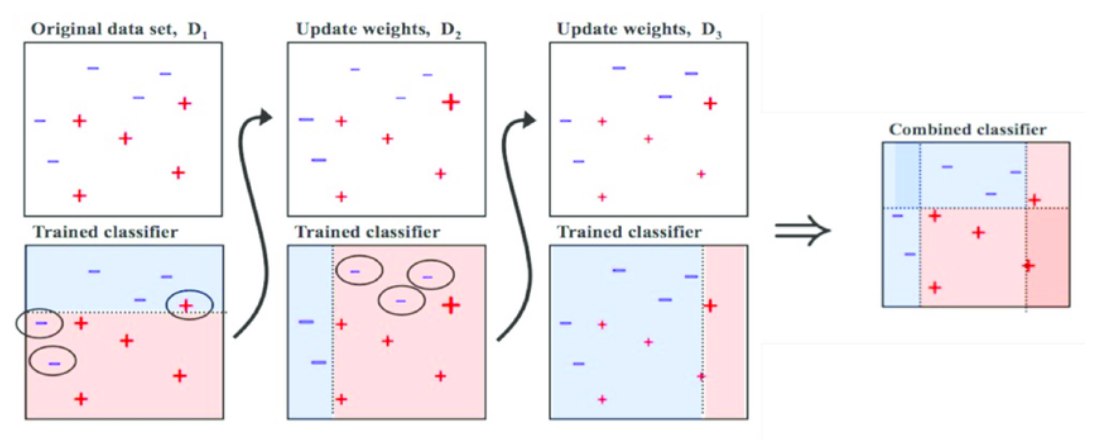
\includegraphics[scale=0.3]{AdaBoost_Schema.png}
\end{center}

Weak learner (or $\gamma$-weak-learner): it's an \textbf{algorithm} returning a function $h$ such that $L_{\mathcal{D}}(h) \leq 1/2 - \gamma$. In other words, it returns a simple binary predictor that does slightly better than a random guess.

\vspace{5mm}

\begin{algorithm}
\caption{AdaBoost}
\begin{algorithmic}
\State Input: training set $S=(x_1,y_1),...,(x_m,y_m)$, weak learner WL, number of rounds $T$
\State Initialize $D^{(1)} = (1/m,...,1/m)$ // same weights for all observations
\For{t = 1,...,T}
\State invoke weak learner $h_t = WL(D^{(t)},S)$
\State compute $\epsilon_t = \Sigma_{i=1}^m D_i^{(t)} \mathbbm{1}_{[y_i \neq h_t(x_i)]}$ // misclassification error
\State let $\omega_t = \frac{1}{2} log(\frac{1}{\epsilon_t}-1)$ // $\epsilon_t < 1$
\State update $D_i^{(t+1)} = \frac{D_i^{(t)} exp(-\omega_t y_i h_t(x_i))}{\Sigma_{j=1}^m D_j^{(t)} exp(-\omega_t y_j h_t(x_j))}$ for all $i=1,...,m$
\EndFor
\State Output: the hypothesis $h_s(x) = sign(\Sigma_{t=1}^T \omega_t h_t (x))$
\end{algorithmic}
\end{algorithm}

We note:

- Final predictor = weighted sum of weak predictors

- More weights are given to observations that gave wrong prediction. In doing so, the classifier of the next round will focus on these observations. Warning: to see this, focus on the variation of $D^{(t+1)}_i$ and not just $w_t$.

\vspace{5mm}

Theorem: the training error of the output hypothesis decreases \textbf{exponentially fast} with the number of boosting rounds.

\vspace{5mm}